\documentclass[a4paper, 10pt]{amsart}
\usepackage[greek, german]{babel}
\languageattribute{greek}{polutoniko}
\usepackage[utf8]{inputenc}
%\usepackage[light]{CormorantGaramond}
%\usepackage[T1]{fontenc}
%\usepackage{microtype}

\usepackage{epigraph}
%\setlength\epigraphwidth{.8\textwidth}
%\setlength\epigraphrule{0pt}

\usepackage{amssymb}
\usepackage{amsthm}
\usepackage{amstext}
\usepackage{amsmath}
\usepackage{amsfonts}
\usepackage{mathtools}

\usepackage{tikz}
\usepackage{tikzit}
\usetikzlibrary{math, decorations.pathreplacing,shapes,calc,fit,decorations.markings,positioning,patterns,arrows.meta,cd,babel}
% TiKZ style file generated by TikZiT. You may edit this file manually,
% but some things (e.g. comments) may be overwritten. To be readable in
% TikZiT, the only non-comment lines must be of the form:
% \tikzstyle{NAME}=[PROPERTY LIST]

\tikzset{->-/.style={decoration={
  markings,
  mark=at position #1 with {\arrow{\arrowstyle[scale=\arrowscale]}}},postaction={decorate}},
   arrow scale/.store in=\arrowscale,
   arrow scale=.8,
   arrow style/.store in=\arrowstyle,
   arrow style={>},}

\tikzset{->/.style={}}

% Node styles
\tikzstyle{red node}=[fill=red, tikzit category=nodes]
\tikzstyle{blue node}=[fill=blue]
\tikzstyle{blue node 2}=[tikzit fill=green, fill=blue]
\tikzstyle{yellow square}=[draw=black, fill=yellow, shape=rectangle]
\tikzstyle{small box}=[fill=white, draw=black, shape=rectangle, minimum width=0.5cm, minimum height=0.5cm, rounded corners=2pt, tikzit category=nodes, thick]
\tikzstyle{medium box}=[fill=white, draw=black, shape=rectangle, minimum width=0.75cm, minimum height=1cm, rounded corners=2pt, tikzit category=nodes, thick]
\tikzstyle{large box}=[fill=white, draw=black, shape=rectangle, tikzit category=nodes, minimum width=0.75cm, minimum height=1.5cm, thick, rounded corners=2pt]
\tikzstyle{small thin box}=[fill=white, draw=black, shape=rectangle, tikzit category=nodes, minimum height=.9cm, thick, inner sep=1pt, minimum width=0pt, rounded corners=2pt]
\tikzstyle{medium thin box}=[fill=white, draw=black, shape=rectangle, minimum height=1.3cm, rounded corners=2pt, tikzit category=nodes, thick, inner sep=1pt, minimum width=0pt]
\tikzstyle{large thin box}=[fill=white, draw=black, shape=rectangle, tikzit category=nodes, minimum height=1.8cm, thick, inner sep=1pt, minimum width=0pt, rounded corners=2pt]
\tikzstyle{tall thin box}=[fill=white, draw=black, shape=rectangle, tikzit category=nodes, thick, minimum height=3cm, inner sep=0.5pt, minimum width=0pt, rounded corners=2pt]
\tikzstyle{thin tall box}=[fill=white, draw=black, shape=rectangle, tikzit category=nodes, thick, minimum height=3cm, inner sep=0.5pt, minimum width=0pt, rounded corners=2pt]

% Edge styles
\tikzstyle{line}=[thick, -]
\tikzstyle{dashed edge}=[<->, dashed]
\tikzstyle{blue pointer}=[->, draw=blue]
\tikzstyle{r-arrow}=[->, thick, ->-=0.999]
\tikzstyle{cent-r-arr}=[thick, ->-=0.5, ->]
\tikzstyle{end-near}=[->, ->-=0.9, thick]
\tikzstyle{begin-near}=[->, thick, ->-=0.2]
\tikzstyle{brace}=[->, decoration={brace, amplitude=10pt}, decorate, thick]
\tikzstyle{sh-brace}=[->, decoration={brace, amplitude=5pt}, thick, decorate]


\usepackage{graphicx}
\usepackage[margin=3.5cm]{geometry}
\renewcommand{\baselinestretch}{1.1}

\usepackage[linktocpage=true]{hyperref}
\usepackage[xspace]{ellipsis}

%Plain style
\theoremstyle{plain}
\newtheorem{defn}{Definition}[section]
\newtheorem{thm}[defn]{Theorem}
\newtheorem{hypo}[defn]{Hypothesis}
\newtheorem{lem}[defn]{Lemma}
\newtheorem{cor}[defn]{Corollary}
\newtheorem{fact}[defn]{Fact}
\newtheorem{prop}[defn]{Proposition}

\begin{document}
\setcounter{tocdepth}{1}
\title{Notizen und Gedanken zu Niklas Luhmann.}
\author{Arne Hofmann}
\date{\today}
\maketitle
\tableofcontents
Die folgenden Stichpunkte, Fragen, Bemerkungen und Verweise beziehen sich auf die gemeinsame Lektüre von Niklas Luhmanns Werk \emph{Soziale Systeme} \cite{luhmann1984soziale} im Früh\-lings\-se\-mes\-ter 2019 in Zürich. In der Sache von Verweisen halte ich mich an die mathematische Konvention, weil ich zu faul und intolerant für andere Konventionen bin.

Die Gedanken und Meinungen, die hier geäußert werden, sind Versuche und Diskussionsansätze, keine Ergebnisse. Caveat lector.
\section{Allgemeine Bemerkungen}
\subsection{Skepsis.}
Luhmann: ``Allgemeinheiten können trivial sein''. Polemisch muss man fast sagen: Allgemeinheiten \emph{m\"ussen} trivial sein. Etwas genauer: alle Sätze, die für eine Klasse $K$ von Objekten gelten, gelten für jede Teilklasse $K'$, kontrapositiv also: für jede Klasse $K'$, die $K$ enthält, gelten bestenfalls alle Aussagen, die für $K$ gelten (im Allgemeinen weniger). Wenn man umfassendere Klassen $K$ betrachtet, lässt sich weniger aussagen.

Der Begriff ``System'' ist a priori so allgemein, dass er praktisch alles umfasst. Über die Eigenschaften eines ganz beliebigen Etwas lässt sich aber überhaupt nichts sagen.

Die einzige Hoffnung für eine ``allgemeine Systemtheorie'' ist also, dass sie ihren Untersuchungsgegenstand wirkungsvoll einschränkt. Das heißt, man muss herausfinden, was \emph{kein} System ist.
\subsection{Noch etwas zur ``reinen Theorie.''}
\label{sec:reine-theorie}
Es gibt keine reine Theorie. Soweit ich weiß, ist die erste Bedeutung von \emph{teoria} die \emph{Anschauung} (die Altphilologen mögen mich korrigieren). Aber es gibt keine Anschauung, ohne etwas, das angeschaut wird.

Ich kehre zu meiner eigenen Disziplin zurück und zitiere einen Giganten unter Mathematikern, William F. Lawvere \cite{InterviewWilliamLawvere}.

\begin{quotation}
Having recognized already in the 1960s that there is no such thing as a heaven-given platonic ``justification'' for mathematics, I tried to give the word ``Foundations'' more progressive meanings in the spirit of Eilenberg and Truesdell. That is, I have tried to apply the living axiomatic method to making explicit the essential features of a science as it is developing in order to help provide a guide to the use, learning, and more conscious development of the science. A ``pure'' foundation which forgets this purpose and pursues a speculative ``foundation'' for its own sake is clearly a NON-foundation. Foundations are derived from applications by unification and concentration, in other words, by the axiomatic method. Applications are guided by foundations which have been learned through education [...]

During the past forty years we have become accustomed to the fact that foundations are relative, not absolute. I believe that even greater clarifications of foundations will be achieved by consciously applying a concentration of applications from geometry and analysis, that is, by pursuing the dialectical relation between foundations and applications.
\end{quotation}

Theorie ist die eine Richtung der \emph{dialektischen Beziehung zwischen Grundlagen und Anwendungen}. Ich behaupt, so etwas wie eine Theorie ohne einen Anwendungsbereich gibt es gar nicht oder verdient nicht den Namen Theorie -- ein Lehrgebäude ohne Wechselspiel zwischen Abstraktion und Konkretisierung ist leer, tot. Und das sage ich, nicht nur obwohl, sondern gerade weil ich ein glühender Verfechter der vielleicht abstraktesten Disziplin der Mathematik, nämlich der Kategorientheorie, bin.

\emph{Anwendung} heißt hier übrigens nicht zwingend \emph{empirische Anwendung}. Im Gegenteil: die Mathematik zeigt (gewissermaßen Paradigmatisch) wie Begriffs- und Theoriebildung ganz ohne Empirie funktionieren kann. Wie die genannte Dialektik in der Mathematik funktioniert, ist sehr klug von Lakatos dargestellt worden \cite{lakatos2015proofs}.
%
\subsection{Antagonismen zur ``klassichen Physik''} An verschiedenen Stellen (wo?) wird die Systemtheorie von der ``klassischen Physik'' abgehoben. Diese klassische Physik sei ``linear'' oder betrachte nur Elemente, nicht jedoch ihre Relationen.

Mit Verlaub: das ist doch wohl Unfug. Man hat ja schon bei ganz einfachen Schaltkreisen in der Elektrodynamik nichtlineare R\"uckkopplung. Das Doppelpendel weist die Empfindlichkeit gegen Anfangsbedingungen auf, die f\"ur ``chaotische Bewegung'' charakteristisch ist. Und die Beziehungen zwischen den Konstituenten eines physikalischen Systems sind ja der Mittelpunkt jeder Analyse.

Aber es gibt nat\"urlich eine Annahme, die praktisch jeder Physik zugrundeliegt. Die Annahme ist, dass man mit Konstituenten (Elementen) arbeiten kann, die \emph{praktisch} (for all practical purposes) strukturlos sind, das hei{\ss}t, keine inneren Zust\"ande haben. Man kann das etwas abschw\"achen, zum Beispiel, wenn es um den Spin (interner Drehimpuls) von Teilchen geht. Aber Spin ist kein komplexes System.

Man betrachtet schon komplexe Systeme, die beliebig starke (ja, auch nichtlineare) Kopplungen (auch Selbst- oder R\"uckkopllungen) aufweisen k\"onnen. Aber die Grundlage f\"ur die Analyse dieser Systeme ist in der Regel doch, dass man sie durch die Wechselwirkung einfacherer Bestandteile beschreiben kann.
%
% Die radikalen Vereinfachungen kommen in zwei Schritten: erstens, dass die Beziehungen der Teilchen untereinander sich nach einem fixen mathematischen Schema (durch Kr\"afte, Potenziale usw.) beschreiben lassen. Das ist noch eine sehr schwache Annahme. Aber um das Problem l\"osbar zu machen, nimmt man dann eine bestimmte Form f\"ur die Potenziale an.
%
% Wie stark man diese Form einschr\"ankt, h\"angt davon ab, ``wieviel L\"osbarkeit'' man haben will. Wenn man Formeln f\"ur die Teilchenbewegung mit elementaren Funktionen aufschreiben will, scheitert man selbst mit Zentralkr\"aften (Keplerproblem) bei drei oder mehr Teilchen. Wenn man numerisch arbeitet, kann man die Teilchenzahl durchaus ein paar Gr\"o{\ss}enordnungen anheben (\cite{kim2011new} simulieren ca. 400 Milliarden Teilchen).
%
% Es gibt kein fundamentales Prinzip der klassischen Physik, das nichtlineare oder komplexe Systeme ausschlie{\ss}en w\"urde. 
\section{Begriffe}
\subsection{System/Umwelt}
Kneer/Nassehi \cite{kneerNiklasLuhmannsTheorie1993} sagen:
\begin{quote}
\emph{System}: Ganzheit einer Menge von Elementen und deren Relation zueinander.
\end{quote}
\subsection{Kommunikation}
Der Begriff \emph{Kommunikation} ist sp\"atestens seit Shannon \cite{shannon1948mathematical} Teil der Mathematik. Daraus ein pr\"agnanter Abschnitt:
\begin{quotation}
The fundamental problem of communication is that of reproducing at one point either exactly or approximately a message selected at another point. Frequently the messages have meaning; that is they refer to or are correlated according to some system with certain physical or conceptual entities.  These semantic aspects of communication are irrelevant to the engineering problem. The significant aspect is that the actual message is one selected from a set of possible messages. The system must be designed to operate for each possible selection, not just the one which will actually be chosen since this is unknown at the time of design.
\end{quotation}
Ich lese dieses Paper gerade (13.5.19) zum ersten Mal, obwohl es in der angewandten Mathematik geradezu ber\"uhmt ist. Die Mathematik ist nicht besonders kompliziert; ich denke, es ist auch f\"ur Geisteswissenschaftler einen Blick wert.

Insbesondere gibt es bei Shannon eine Abbildung (Abbildung \ref{fig:shannon-1}), die ziemlich genau dem entspricht, was ich in der heutigen Diskussion skizziert habe (bevor ich mir den Artikel angeguckt hatte).

\begin{figure}
\centering
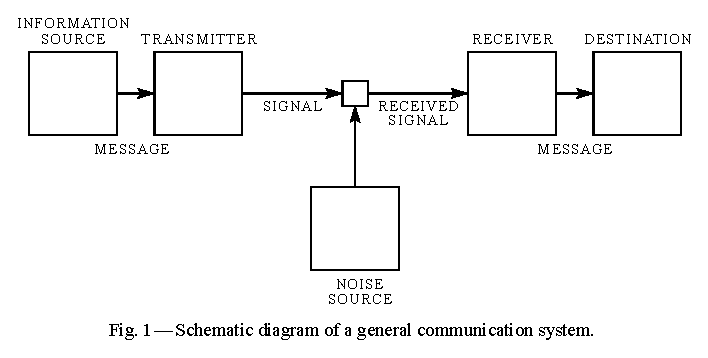
\includegraphics[width=0.6\textwidth]{figures/shannon-1.eps}
\caption{Abbildung aus \cite{shannon1948mathematical}.\label{fig:shannon-1}}
\end{figure}

Es gibt jedoch auch Unterschiede. Shannon interessiert sich nur f\"ur explizite Nachrichten, die nach einem vereinbarten System verschickt werden. Das hei{\ss}t zum Beispiel auch, dass der \emph{Receiver} einfach die inverse Operation zum \emph{Transmitter} ausf\"uhrt. Luhmann will offenbar auch subtilere Arten der Kommunikation behandeln (K\"orpersprache, Gesichtsausdr\"ucke, unklarer Sprachgebrauch usw.).

\emph{Arbeitshypothese}: man kann allgemeinere menschliche Kommunikation in die Abbildung \ref{fig:shannon-1} integrieren, indem man die Arbeitsweisen von Transmitter und Empf\"anger als variabel und abh\"angig von einem psychischen System (Mensch) betrachtet.

Unter diesen Umst\"anden ist es erst einmal sinnvoll, davon auszugehen, dass es keine St\"orung in der \"Ubertragung gibt. Dann haben wir einfach eine Operation des Transmitters, $\phi$, und eine des Empf\"angers, $\phi'$. Damit eine Botschaft $A$ perfekt \"ubertragen wird, muss
\begin{align}
\phi'(\phi(A)) = A
\end{align}
sein. Damit dies f\"ur beliebige Botschaften $A$ gilt, muss $\phi'$ gerade die inverse Operation zu $\phi$ sein.

Wenn $\phi$ und $\phi'$ variabel sind, ist perfekte Kommunikation also nur unter sehr besonderen Umst\"anden m\"oglich. Es muss irgendwie zumindest eine grobe Art Einigung hergestellt werden, \emph{wie man miteinander kommuniziert}. Wie soll das geschehen, wenn nicht per Kommunikation? Da haben wir schon unser rekursives Element!

Wir wollen ein paar erste Definitionen versuchen, die allerdings \"uberhaupt nicht so pr\"azise sind, wie sie vielleicht auf den ersten Blick aussehen. Man darf nicht vergessen, dass die Operationen des Transmitters vom \emph{Zustand eines psychischen Systems abh\"angig sein sollen}. Das ist noch nicht richtig zum Ausdruck gebracht.
\begin{defn} Ein \emph{Kommunikator} $T$ ist gleichzeitig ein Transmitter und ein Empf\"anger. Die \emph{Sendeoperation} von $T$ schreiben wir als $\phi_T$ und die \emph{Empf\"angeroperation} als $\psi_T$. 
\end{defn}
\begin{defn} Sei $\mathcal{A}$ eine Sprache und $A \in \mathcal{A}$ ein Wort. Seien ferner $T_1, T_2$ Kommunikatoren. Eine \emph{Kommunikation von} $T_1$ \emph{zu} $T_2$ ist ein Paar $(A, \psi_{T_2}(\phi_{T_1}(A)))$.
\end{defn}
Vielleicht nennen wir dieses Konzept besser eine \emph{\"Ubertragung} -- und sprechen nur von \emph{Kommunikation}, wenn $A \approx \psi_{T_2}(\phi_{T_1}((A))$ (ungef\"ahr gleich)?

Dann k\"onnen wir n\"ahmlich eine Grenze oder \emph{Differenz} herstellen (und damit Luhmanns gr\"o{\ss}te Sehnsucht befriedigen) -- zwischen Kommunikationen und \"Ubertragungen, die keine Kommunikationen sind. Diese Differenz h\"angt einerseits entscheidend von den psychischen Systemen ab, an denen die ganze \"Ubertragung h\"angt, muss andererseits selber durch Kommunikation hergestellt werden (man kommuniziert dar\"uber, wie man kommunizieren kann).

Ich sehe jedoch nicht, wie sich hier das System der Kommunikationen gegen die psychischen Systeme absetzt, die nach Luhmann ja die \emph{Umwelt} des Kommunikationssystems bilden sollen.
\subsection{Komplexit\"at}
\subsection{Elemente}
\section{Beispiele}
\subsection{Wieso Beispiele?} 
Man beachte folgende Zitate von Paul Halmos:
\begin{quotation}
$\quad \bullet$ Don't just read it; fight it! Ask your own questions, look for your own examples, discover your own proofs. Is the hypothesis necessary? Is the converse true? What happens in the classical special case? What about the degenerate cases? Where does the proof use the hypothesis?

$\bullet$ [..] the source of all great mathematics is the special case, the concrete example. It is frequent in mathematics that every instance of a concept of seemingly great generality is in essence the same as a small and concrete special case.

$\bullet$ A good stack of examples, as large as possible, is indispensable for a thorough understanding of any concept, and when I want to learn something new, I make it my first job to build one.
\end{quotation}
Ich erwähne das hier weil wir über die Legitimität oder den Wert von Beispiel gesprochen haben. Das hängt natürlich mit dem Bild von Theorie zusammen, das ich in Abschnitt \ref{sec:reine-theorie} propagiert habe.

\subsection{Beispiele aus der Mathematik -- Allgemeines.}
Jedenfalls gibt es keine andere Möglichkeit, schwierige Ideen zu verstehen, als sie mit den eigenen Werkzeugen zu zerlegen und zu rekonstruieren. Das ist meine Rechtfertigung dafür, die Mathematik ins Spiel zu bringen.

Ich verlange nicht, dass sich der Gehalt der Systemtheorie ausschließlich auf mathematische Konstruktionen reduzieren lasse. Aber wenn die Systemtheorie ihrem Allgemeinheitsanspruch gerecht werden will, müssen sich ihre Begriffe auch auf mathematische Modelle beziehen lassen. Am Schluss kann man vielleicht nichts so präzises sagen wie: ``der Begriff $X$ der Systemtheorie hat als Spezialfall die mathematische Definition $X'$ im Fall der Modellklasse $Y$'', aber ich würde es als schweren Schlag gegen die Systemtheorie werten, wenn es grundsätzlich nicht möglich wäre, mathematische Modelle zu finden, von denen man sagen könnte: ``die mathematische Definition $X$ umfasst und präzisiert wesentliche Aspekte des Begriffs $X'$ der Systemtheorie.''

\subsection{Beispiele aus der Mathematik -- Kategorientheorie.}
Ich denke hier vor allem an die Arbeiten von Fong \cite{fongCategoricalApproachOpen2016,fongAlgebraOpenInterconnected2016,fongBehavioralMereology2018}, Spivak \cite{spivakOperadWiringDiagrams2013} und Baez \cite{baezCategoriesControl2014} (siehe auch Baez' Bibliographie zur Theorie der Netzwerke, \cite{NetworkTheoryBaez}).
\section{Kapitel/Textstellen}
\subsection{Kombination und Rekombination.}
\emph{Die Aufgabe ist dann, schon vorhandene Texte zu sezieren, zu exegieren, zu rekombinieren.} (SS S. 7). Oder auch (U. Eco, \emph{Das Foucaultsche Pendel}):
\begin{quotation}
In den Versammlungen konnte ich mich nicht f\"ur die Ideologiedebaten erw\"armen, die zwischen den verschiedenen Gruppen gef\"uhrt wurden -- ich hatte immer den Verdacht, da{\ss} es gen\"ugen w\"urde, das richtige Zitat zu finden, um aus der einen in die andere Gruppe zu wechseln. Ich am\"usierte mich mit der Suche nach dem richtigen Zitat. Ich modulierte.
\end{quotation}
\subsection{Erkenntnistheorie.}
Zur Kritik der Erkenntnistheorie suche ich noch eine Stelle aus Gellner \cite{gellner1979legitimation}. Vielleicht folgende:
%
\begin{quotation}
There is perhaps no escaping the argument from regress. If our foundations are well founded they are not ultimate (and we `really' have some others), and if they are not well founded they would seem arbitrary. But the force of this argument, which springs from the fact that fundamental norms are \emph{fundamental}, and not at all from the fact that they are \emph{norms}, should not be confused, as so often it is, with the quite mistaken view that norms are inherently matters of emotion. This conclusion (and its variants, to the effect that they are `only' decisions, prescriptions, and so on) was in any case only reached by a mistaken argument from elimination (`what else could they be?').
\end{quotation}
%
Der Versuch, ``endgültige'' Grundlagen einer Wissenschaft zu finden, führt fast notwendig zur Zirkularität. Man sollte daher die Endgültigkeit der Grundlagen aufgeben und sich ganz der \emph{Dialektik von Grundlagen und Anwendungen} hingeben.
\subsection{Knecht und Herr.} Diese Stelle fand ich frappierend (SS S. 36/37):
\begin{quotation}
Eine der wichtigsten Konsequenzen des System/Umwelt-Paradigmas ist: daß man zwischen der \emph{Umwelt} eines Systems und \emph{Systemen in der Umwelt} dieses Systems unterscheiden muß. Diese Unterscheidung hat eine kaum zu überschätzende Bedeutung. So muß man vor allem die Ab\-häng\-ig\-keits\-be\-zieh\-ung\-en zwischen Umwelt und System unterscheiden von den Ab\-häng\-ig\-keits\-be\-zieh\-ung\-en zwischen Systemen. Diese Unterscheidung torpediert die alte Herr\-schaft/Knecht\-schaft-Thematik. Ob und wie weit sich Verhältnisse ausbilden lassen, in denen ein System ein anderes dominiert, ist nicht zuletzt abhängig davon, wie weit beide Systeme und wie weit das System ihrer Beziehungen von der jeweiligen Umwelt abhängen. In diesem Sinne war denn auch die ``absolute'' Herrschaft, von der ältere Reichsmodelle ausgingen, nie starke, nie determinierende Herrschaft, sondern mehr ein Modus der Systembeschreibung, der eine gewisse Verfügungsgewalt des Systems über sich selbst zum Ausdruck brachte.
\end{quotation}
Vergleiche mit S. 23 in \cite{kneerNiklasLuhmannsTheorie1993}. Dort geht es um den Thermostat, der die Heizung einschaltet, wenn die Raumtemperatur unter einen Richtwert fällt, und über einer bestimmten Temperatur wieder abstellt. Auf den ersten Blick kontrolliert der Thermostat die Temperatur, aber man kann auch sagen, dass die Temperatur das Verhalten des Thermostats kontrolliert.
\begin{quotation}
Man sieht, daß das Kontrollierte auf den Kontrolleur zurückwirkt. Die klassische Kybernetik nennt dies einen \emph{Rückkopplungseffekt} (vgl. Wiener 1963). Neuere kybernetische Arbeiten (``second-order-cybernetics'') versuchen darüber hinaus zu zeigen, daß man Kontrolleur und Kontrolliertes nicht eindeutig voneinander scheiden kann, sondern daß sich die unterschiedlichen Elemente - in unserem Beispiel Thermostat und Raumtemperatur - wechselseitig kontrollieren.
\end{quotation}
Wir können auch ein abstraktes ``Rückkopplungsdiagramm'' aufstellen:
\begin{figure}
\centering
\tikzfig{rueckkopplung}
\caption{Das System $A$ wirkt durch den Mechanismus $f$ auf $B$, umgekehrt wirkt $B$ durch $g$ auf $A$.}
\end{figure}
Per Konstruktion hat das Diagramm eine gewisse Symmetrie; man kann jedenfalls nicht ohne weiteres sagen, dass es einen Kontrolleur und ein kontrolliertes System gibt.

Aber die Beschaffenheit von $f$ und $g$ könnte diese Asymmetrie herstellen. Mehr kann man aus abstrakter Sicht nicht sagen.

Aber um zur eigentlichen Frage zurückzukehren: mir ist nicht klar, auf wen Luhmann hier eigentlich schießt. Damit die Systemtheorie überhaupt relevant sein kann, kann ja nicht die Rede sein vom Verhältnis des einzelnen Knechts zu seinem Herrn (oder umgekehrt), sondern allenfalls von einer ``Gesamtheit'' der Herren und einer ``Gesamtheit'' der Knechte. Ich stelle Gesamtheit in Anführungszeichen, weil es doch nicht klar ist, ob diese Gruppen überhaupt Einheiten darstellen, die Beziehungen zueinenander herstellen können, die über die individuellen Beziehungen hinausgehen.
\bibliographystyle{amsalpha}
\bibliography{literatur}
\end{document}